\documentclass{article}

\usepackage{hyperref}
\hypersetup{
    colorlinks=true,
    linkcolor=blue,
    filecolor=magenta,      
    urlcolor=cyan,
}

% for including notebooks
\usepackage{pdfpages}
\usepackage{fancyhdr}
\usepackage{extramarks}
\usepackage{amsmath}
\usepackage{amsthm}
\usepackage{amsfonts}
\usepackage{tikz}
\usepackage{float}
\usepackage[plain]{algorithm}
\usepackage{algpseudocode}
\usepackage{caption}
\usepackage{subcaption}
\usepackage[toc,page]{appendix}
\usepackage{siunitx}
\usepackage{footnote}

\usepackage{listings}
\usepackage{color} 
\definecolor{mygreen}{RGB}{28,172,0} 
\definecolor{mylilas}{RGB}{170,55,241}

\lstset{
    basicstyle=\scriptsize\sffamily\color{black},
    frame=single,
    numbers=left,
    showspaces=false,
    showstringspaces=false,
    tabsize=1
}
\lstset{language=Matlab,%
    %basicstyle=\color{red},
    breaklines=true,%
    morekeywords={matlab2tikz},
    keywordstyle=\color{blue},%
    morekeywords=[2]{1}, keywordstyle=[2]{\color{black}},
    identifierstyle=\color{black},%
    stringstyle=\color{mylilas},
    commentstyle=\color{mygreen},%
    showstringspaces=false,%without this there will be a symbol in the places where there is a space
    numbers=left,%
    numberstyle={\tiny \color{black}},% size of the numbers
    numbersep=9pt, % this defines how far the numbers are from the text
    emph=[1]{for,end,break},emphstyle=[1]\color{red}, %some words to emphasise
    %emph=[2]{word1,word2}, emphstyle=[2]{style},    
}

\topmargin=-0.45in
\evensidemargin=0in
\oddsidemargin=0in
\textwidth=6.5in
\textheight=9.0in
\headsep=0.25in


\linespread{1.1}

\pagestyle{fancy}
\fancyhf{}
\lhead{\hmwkAuthorName}
\chead{\hmwkClass: \hmwkTitle}
\rhead{\leftmark}
\lfoot{\lastxmark}
\cfoot{\thepage}

\renewcommand\headrulewidth{0.4pt}
\renewcommand\footrulewidth{0.4pt}

\setlength\parindent{0pt}

\newcommand{\hmwkTitle}{Assignment \ 2}
\newcommand{\hmwkDueDate}{April 27, 2020}
\newcommand{\hmwkClass}{Introduction to AI}
\newcommand{\hmwkClassInstructor}{Dr. Joseph Brown}
\newcommand{\hmwkAuthorName}{\textbf{Artem Bakhanov (B18-03)}}

%
% Title Page
%

\title{
    \vspace{2in}
    \textmd{\textbf{\hmwkClass:\ \hmwkTitle}}\\
    \normalsize\vspace{0.1in}\small{Due\ on\ \hmwkDueDate\ at 11:59pm}\\
    \vspace{0.1in}\large{\textit{\hmwkClassInstructor\ }}
    \vspace{3in}
}

\author{\hmwkAuthorName}
\date{}

\begin{document}

\maketitle

\pagebreak

\tableofcontents

\pagebreak

\section{Introduction}
\subsection{General information}
    The assignment is solved by me, Artem Bakhanov, a student of Innopolis University. If you have any question regarding any part of this document and other provided materials, you can contact me via email: \href{mailto:a.bahanov@innopolis.university}{a.bahanov@innopolis.university}.\\
    In this assignment, I used Python 3.7 as a programming language. Also OpenCV and Numpy were used to work with images easily and with high performance. For generating Voronoi polygons I used Scipy. All files with code are in directory \texttt{/code}.
\subsection{Running the code}
First of all, you need to install Python of version 3.7. Note, that the code was not tested on Python 3.8, I cannot guarantee it works on Python 3.8. Install dependencies with \texttt{pip install -r requirements.txt} (this command may vary on different OSs and computers). Then you can run \texttt{main.py} and it will generate some image. If you want another image or you want to change parameters - edit \texttt{main.py} file. 

\section{The Story}
In the beginning I had a lot of ideas which were about generating triangles or more complex polygons to recreate the original image. Initially, I created a program that did it but I did not like the result I got. I started researching and probing a lot. For now I created about 6 different algorithms and I was not satisfied with any of them. The problem was that it was too edgy and "sharp". The images I got were just inaccurate replica of the original images. So I decided that randomness in the figures is not cool and I remembered my internship in 2019 when I was creating an app that reconstructs 3d mesh. One of the task that I needed to solve - Voronoi Partition. This algorithm gives really beautiful images. I took the algorithm and I took one my idea from the previous algorithm - RGB splitting. My final program creates image out of 3 independent Voronoi Diagrams - each in separate color layer. And the result is interesting. It is structured and chaotic at the same time.

\section{Representation}
This section is about representation of the algorithm.
\subsection{Genetic Algorithm}
For this part, I created my own module "ga" that should work with any entities you want. All that is needed is to follow the templates and use the base classes. It provides different types of mutation, selection and crossover algorithms. I created it for my own convenience so that I can easily play with parameters.

To start genetic algorithm, you need to create your own generator class inherits \texttt{Generator} class for the module. Also you need to adjust parameters (e.g. selection algorithm, population size, etc.)
\subsection{Image representation}
\begin{figure}[ht]
   	 \centering
     \begin{subfigure}[b]{0.45\textwidth}
         \centering
         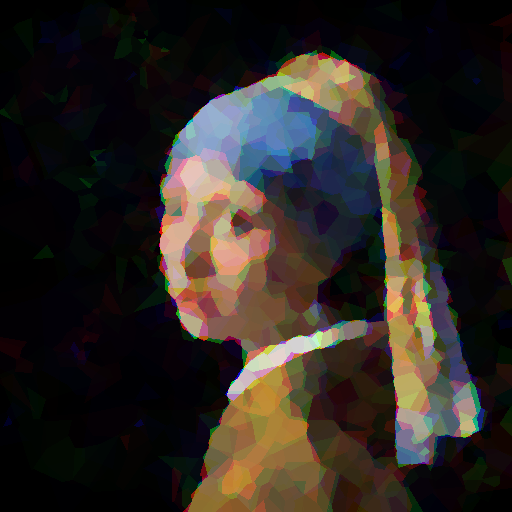
\includegraphics[width=\textwidth]{latex_src/voronoi18.png}
         \caption{Final Result}
     \end{subfigure}
     \hfill
     \begin{subfigure}[b]{0.45\textwidth}
         \centering
         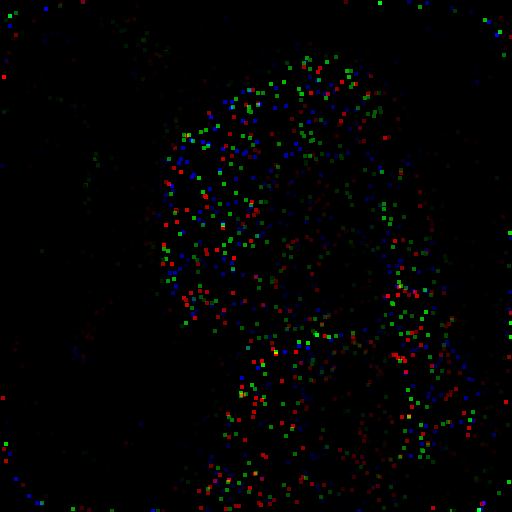
\includegraphics[width=\textwidth]{latex_src/voronoi18_1.png}
         \caption{Centers of Polygons}
     \end{subfigure}
      \caption{Generation 500,000. Result and centers.}
\end{figure}
In my code Image is represented as class with 3 layers - arrays of "centers" of polygons and their color (a number between 0 and 255). The number of points in each layer is 1369; it was adjusted by hands. These 3 layers are the genome of the image. On the figures you can see how the image is represented.
\begin{figure}[ht]
   	 \centering
     \begin{subfigure}[b]{0.3\textwidth}
         \centering
         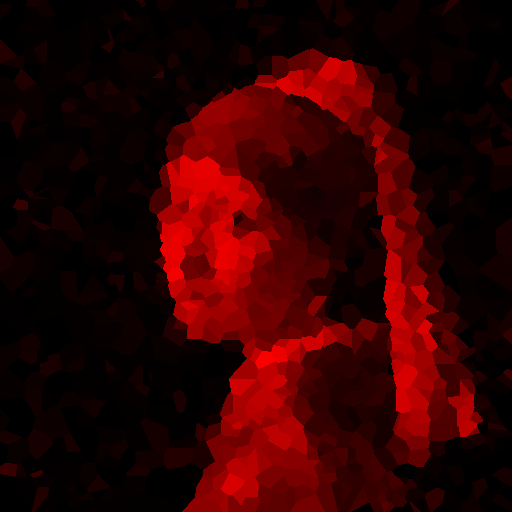
\includegraphics[width=\textwidth]{latex_src/r.png}
         \caption{Red Layer}
     \end{subfigure}
     \hfill
     \begin{subfigure}[b]{0.3\textwidth}
         \centering
         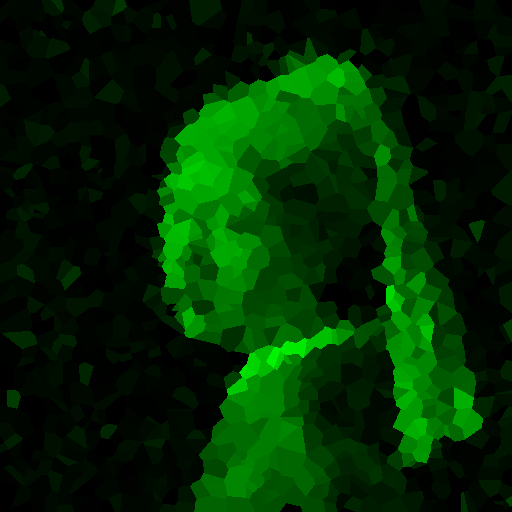
\includegraphics[width=\textwidth]{latex_src/g.png}
         \caption{Green Layer}
     \end{subfigure}
     \hfill
     \begin{subfigure}[b]{0.3\textwidth}
         \centering
         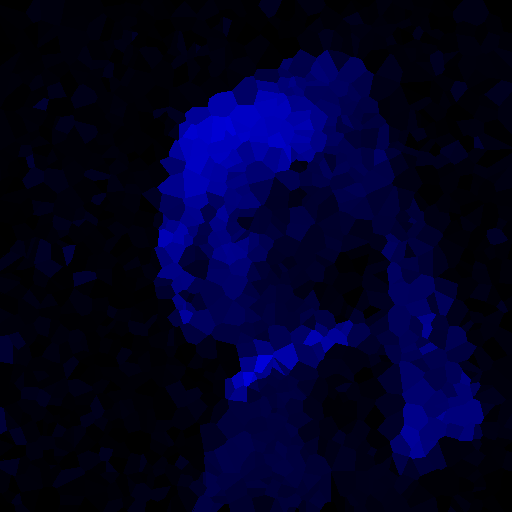
\includegraphics[width=\textwidth]{latex_src/b.png}
         \caption{Blue Layer}
     \end{subfigure}
     \caption{Generation 168842. Layers of the Image}
\end{figure}
\section{Population}
This paragraph is about the size of population. I tested my algorithm on a big number of tests and I got to a conclusion: there is no need to generate more than 1 entity in one population. I tried to change a lot of parameters but it did not change the overall image and I can explain why it happens. My image is generated using polygons and the number of polygons are plus or minus is constant (the number can change because the Voronoi polygons can generate polygons that are impossible to draw). For this reason everytime we will get different images in genome but they will look very similar for a human eye. Yes, genotype is different but for humans only phenotype is important. Another problem was convergence of the population to one good result. I tried different techniques described in the following paragraphs but it did not yield any improvements. For this reason I did not use any crossover function. Every iteration (generation) two mutated kids are generated and selection algorithm is applied. The artistic results became better due to this improvement. Below you can see three images. two of them were generated using only mutations and one with population size = 10, 2 point crossover. The results (phehotypes) are very similar. Since I do not use any crossover function, I do not use parent selection algorithm. But I tried panmixis and random outbreeding. Random outbreeding was more effective in terms of generating diverse genotypes. But eventually the diversity of the genotype was really small (on big number of populations).
\section{Selection Algorithm}
My algorithm need to choose one individual out of several mutated individuals and one individual from the previous generation. My experiments showed that the best solution is truncation selection. The algorithm choose the best individual in terms of the results of the fitness function. 


\section{Image Manipulations}
I do not make any specific image manipulations. I read the image from the memory and do not change it. For the image reading and writing I used opencv library. When I generate image (for example I use it in the fitness function), I use cv2 drawing function \texttt{fillPoly}. Initially, I generate three empty (black) 1-channel images for each layer. Then I iteratively draw the polygons and then I merge the layers using \texttt{cv2.merge} function. 

\section{Fitness function}
Fitness function I use is Mean Squared Error. Initially, I used \texttt{mean\_squared\_error} from \textbf{sklearn} but it was very slow. For this reason, I decided to optimize the fitness function. First of all, I started using \textbf{numba} for optimizing my code. I was forced to write my own mse function. Numba allows very nice optimizations for 1-dimensional arrays and for-loops. Overall I improved the performance in 16 times. Note: the smaller the value of fitness function - the better result.
\begin{lstlisting}[language=Python]
@njit(fastmath=True, parallel=True)
def mse(im1, im2):
    im1 = im1.reshape((1, -1))
    im2 = im2.reshape((1, -1))
    mse = 0
    for i in prange(im1.shape[1]):
        el1 = im1[0, i]
        el2 = im2[0, i]
        mse += (el1 - el2) ** 2

    return mse / im1.shape[1]
\end{lstlisting}

\section{Mutation}
Mutation has 100\% chance to happen. It is one point mutation: one layer is selected, one point is selected and either x-, y-coordinate, or it's color is changed. The probability to select a channel is $\frac{1}{3}$; to change x- or y-coordinate before generation 50,000 - 50\%; after it decreases till 0\% linearly at generation 150,000.
This probabilities were obtained during several experiments. I estimated performance time and the output image. These parameters seemed to me appropriate.

\section{What is art for me?}
Art is a very simple word and a very difficult concept. Every person can define it in their own way so some readers might not agree with in this paragraph. For me art is something that is created by a human, a machine, or even by an animal. It is created for conveying creator's feelings, experience which sometimes cannot be expressed using words. This feelings should be visible by a spectator, or audible by a listener, or even touchable. How the feelings of the creator are understood is also art. Everyone can see different things in some piece of art because they try to find the piece of themselves. They are co-authors. For some authors it is important that spectators feel what they wanted them to feel, some creators leave space for thoughts. Another import thing about art is that is not soullessly created. This is why a lot of people go to galleries or museums. Even if a piece of art is created by machine, someone put their heart into the program. It is also meaningful.
\section{Artistic Value}
I treat images that are generated by my algorithm for several reasons.\\
\textbf{Firstly}, an idea that 3 independent layers can create some meaningful image make me think about structure and chaos in the universe. Just think how you can represent the image, made it and the image will look how you want. It will be structured and chaotic at the same time (look at borders - they are "glitchy" but in a good way). \\
\textbf{Secondly}, it shows human potentials. What can you see on the images generated with a machine? You even can find something in the image that at first look seems to be very random and meaningless. The works of my algorithm shows that human's brain and eyes are very complicated and deserve more attention. \\
\textbf{Thirdly}, it is the algorithm that more or less simulates simple evolution. It shows that actually randomness can help to reach some goals in a very big search space. Evolutionary algorithms are very powerful ones since one of them (but really complicated) created us, humans! What were the chances?..
\section{Performance}
\subsection{Time performance}
Time performance is very poor due to very slow function that generates Voronoi Polygons (from scipy). Image usually starts converging at 10,000 generation (shape is visible from medium distance). It takes about 2 minutes. After generation 90,000 the algorithm works faster since the points are not moved after that and voronoi diagram is not calculated every time.
\subsection{Memory performance}
The program does not consume memory. It takes about 1-30 MB to run.

\section{Examples}
Below you can find some examples. All of them are 180,000 - 200,000 generations (except for the first one: 500,000). Every picture was obtained in 15-20 minutes (IntelCore i7 7th gen.)
\begin{figure}[ht]
   	 \centering
     \begin{subfigure}[b]{0.45\textwidth}
         \centering
         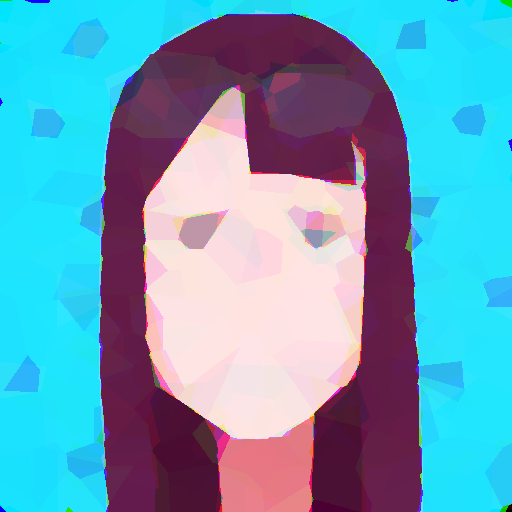
\includegraphics[width=\textwidth]{latex_src/voronoi6.png}
         \caption{Kanamori Sayaka}
     \end{subfigure}
     \hfill
     \begin{subfigure}[b]{0.45\textwidth}
         \centering
         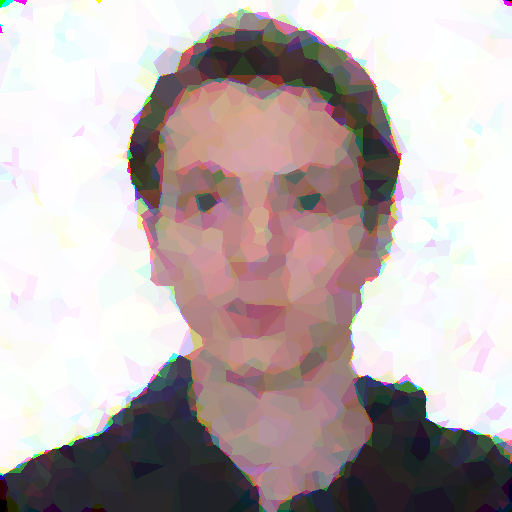
\includegraphics[width=\textwidth]{latex_src/voronoi19.png}
         \caption{Me}
     \end{subfigure}
\end{figure}

\begin{figure}[ht]
   	 \centering
     \begin{subfigure}[b]{0.45\textwidth}
         \centering
         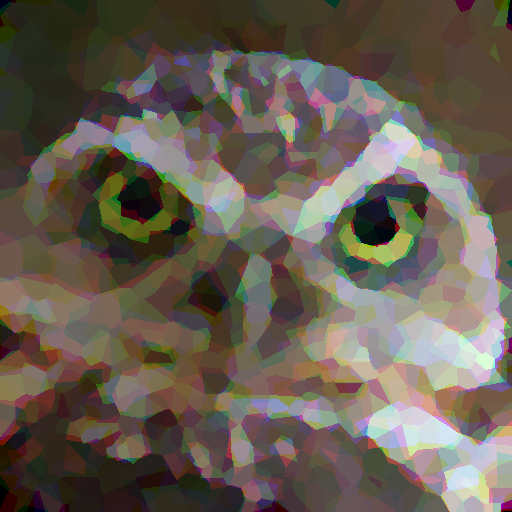
\includegraphics[width=\textwidth]{latex_src/voronoi21.png}
         \caption{Owl}
     \end{subfigure}
     \hfill
     \begin{subfigure}[b]{0.45\textwidth}
         \centering
         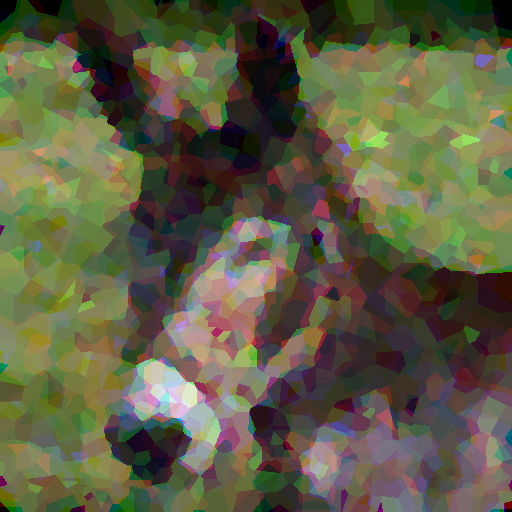
\includegraphics[width=\textwidth]{latex_src/voronoi22.png}
         \caption{Donkey}
     \end{subfigure}
\end{figure}

\begin{figure}[ht]
   	 \centering
     \begin{subfigure}[b]{0.45\textwidth}
         \centering
         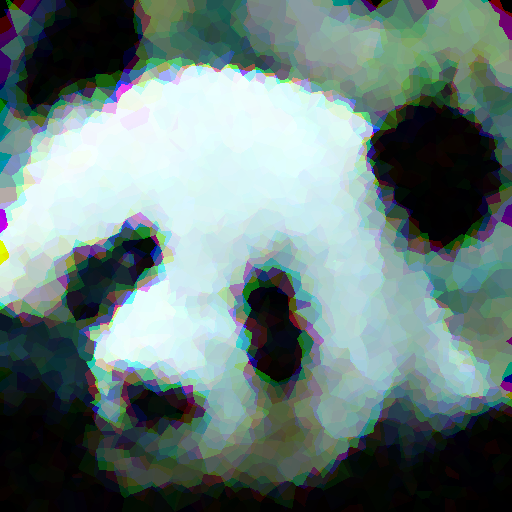
\includegraphics[width=\textwidth]{latex_src/voronoi24.png}
         \caption{Panda}
     \end{subfigure}
     \hfill
     \begin{subfigure}[b]{0.45\textwidth}
         \centering
         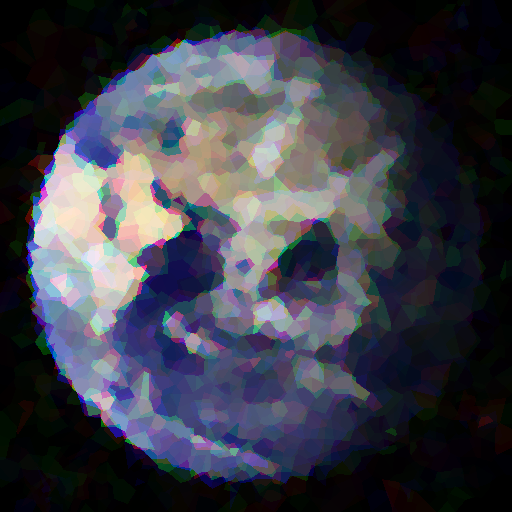
\includegraphics[width=\textwidth]{latex_src/voronoi26.png}
         \caption{The Earth}
     \end{subfigure}
\end{figure}

\begin{figure}[ht]
   	 \centering
     \begin{subfigure}[b]{0.45\textwidth}
         \centering
         
\includegraphics[width=\textwidth]{latex_src/voronoi27.png}
         \caption{Apple Logo (1977)}
     \end{subfigure}
     \hfill
     \begin{subfigure}[b]{0.45\textwidth}
         \centering
         
\includegraphics[width=\textwidth]{latex_src/voronoi28.png}
         \caption{Innopolis Logo}
     \end{subfigure}
\end{figure}

\end{document}

